% This work is licensed under the Creative Commons
% Attribution-NonCommercial-ShareAlike 4.0 International License. To view a copy
% of this license, visit http://creativecommons.org/licenses/by-nc-sa/4.0/ or
% send a letter to Creative Commons, PO Box 1866, Mountain View, CA 94042, USA.

\documentclass[12pt,a4paper]{article} 

% This work is licensed under the Creative Commons
% Attribution-NonCommercial-ShareAlike 4.0 International License. To view a copy
% of this license, visit http://creativecommons.org/licenses/by-nc-sa/4.0/ or
% send a letter to Creative Commons, PO Box 1866, Mountain View, CA 94042, USA.

% PACKAGES
\usepackage[english, ngerman]{babel}	% Paket für Sprachselektion, in diesem Fall für deutsches Datum etc
\usepackage[utf8]{inputenc}	% Paket für Umlaute; verwende utf8 Kodierung in TexWorks 
\usepackage[T1]{fontenc} % ö,ü,ä werden richtig kodiert
\usepackage{amsmath} % wichtig für align-Umgebung
\usepackage{amssymb} % wichtig für \mathbb{} usw.
\usepackage{amsthm} % damit kann man eigene Theorem-Umgebungen definieren, proof-Umgebungen, etc.
\usepackage{mathrsfs} % für \mathscr
\usepackage[backref]{hyperref} % Inhaltsverzeichnis und \ref-Befehle werden in der PDF-klickbar
\usepackage[english, ngerman, capitalise]{cleveref}
\usepackage{graphicx}
\usepackage{grffile}
\usepackage{setspace} % wichtig für Lesbarkeit. Schöne Zeilenabstände

\usepackage{enumitem} % für custom Liste mit default Buchstaben
\usepackage{ulem} % für bessere Unterstreichung
\usepackage{contour} % für bessere Unterstreichung
\usepackage{epigraph} % für das coole Zitat

\usepackage{tikz}

% This work is licensed under the Creative Commons
% Attribution-NonCommercial-ShareAlike 4.0 International License. To view a copy
% of this license, visit http://creativecommons.org/licenses/by-nc-sa/4.0/ or
% send a letter to Creative Commons, PO Box 1866, Mountain View, CA 94042, USA.

% THEOREM-ENVIRONMENTS

\newtheoremstyle{mystyle}
  {20pt}   % ABOVESPACE \topsep is default, 20pt looks nice
  {20pt}   % BELOWSPACE \topsep is default, 20pt looks nice
  {\normalfont} % BODYFONT
  {0pt}       % INDENT (empty value is the same as 0pt)
  {\bfseries} % HEADFONT
  {}          % HEADPUNCT (if needed)
  {5pt plus 1pt minus 1pt} % HEADSPACE
	{}          % CUSTOM-HEAD-SPEC
\theoremstyle{mystyle}

% Definitionen der Satz, Lemma... - Umgebungen. Der Zähler von "satz" ist dem "section"-Zähler untergeordnet, alle weiteren Umgebungen bedienen sich des satz-Zählers.
\newtheorem{satz}{Satz}[section]
\newtheorem{lemma}[satz]{Lemma}
\newtheorem{korollar}[satz]{Korollar}
\newtheorem{proposition}[satz]{Proposition}
\newtheorem{beispiel}[satz]{Beispiel}
\newtheorem{definition}[satz]{Definition}
\newtheorem{bemerkungnr}[satz]{Bemerkung}
\newtheorem{theorem}[satz]{Theorem}

% Bemerkungen, Erinnerungen und Notationshinweise werden ohne Numerierungen dargestellt.
\newtheorem*{bemerkung}{Bemerkung.}
\newtheorem*{erinnerung}{Erinnerung.}
\newtheorem*{notation}{Notation.}
\newtheorem*{aufgabe}{Aufgabe.}
\newtheorem*{lösung}{Lösung.}
\newtheorem*{beisp}{Beispiel.} %Beispiel ohne Nummerierung
\newtheorem*{defi}{Definition.} %Definition ohne Nummerierung
\newtheorem*{lem}{Lemma.} %Lemma ohne Nummerierung


% SHORTCUTS
\newcommand{\R}{\mathbb{R}}				 % reelle Zahlen
\newcommand{\Rn}{\R^n}						 % der R^n
\newcommand{\N}{\mathbb{N}}				 % natürliche Zahlen
\newcommand{\Z}{\mathbb{Z}}				 % ganze Zahlen
\newcommand{\C}{\mathbb{C}}			   % komplexe Zahlen
\newcommand{\gdw}{\Leftrightarrow} % Genau dann, wenn
\newcommand{\with}{\text{ mit }}   % mit
\newcommand{\falls}{\text{falls }} % falls
\newcommand{\dd}{\text{ d}}        % Differential d

% ETWAS SPEZIELLERE ZEICHEN
%disjoint union
\newcommand{\bigcupdot}{
	\mathop{\vphantom{\bigcup}\mathpalette\setbigcupdot\cdot}\displaylimits
}
\newcommand{\setbigcupdot}[2]{\ooalign{\hfil$#1\bigcup$\hfil\cr\hfil$#2$\hfil\cr\cr}}
%big times
\newcommand*{\bigtimes}{\mathop{\raisebox{-.5ex}{\hbox{\huge{$\times$}}}}} 

% WHITESPACE COMMANDS
%non-restrict newline command
\newcommand{\enter}{$ $\newline} 
%praktischer Tabulator
\newcommand\tab[1][1cm]{\hspace*{#1}}

% TEXT ÜBER ZEICHEN
%das ist ein Gleichheitszeichen mit Text darüber, Beispiel: $a\stackeq{Def} b$
\newcommand{\stackeq}[1]{
	\mathrel{\stackrel{\makebox[0pt]{\mbox{\normalfont\tiny #1}}}{=}}
} 
%das ist ein beliebiges Zeichen mit Text darüber, z. B.  $a\stackrel{Def}{\Rightarrow} b$
\newcommand{\stacksymbol}[2]{
	\mathrel{\stackrel{\makebox[0pt]{\mbox{\normalfont\tiny #1}}}{#2}}
} 

% UNDERLINE
% besseres underline 
\renewcommand{\ULdepth}{1pt}
\contourlength{0.5pt}
\newcommand{\ul}[1]{
	\uline{\phantom{#1}}\llap{\contour{white}{#1}}
}


% hier noch ein paar Commands die nur ich nutze, weil ich sie mir im Laufe der Jahre angewöhnt habe und sie mir jetzt nicht abgewöhnen will:

\newcommand{\gdw}{\Leftrightarrow}   % genau dann, wenn




\author{Willi Sontopski}

\parindent0cm %Ist wichtig, um führende Leerzeichen zu entfernen

\usepackage{pdflscape}
\usepackage{rotating}
\usepackage{scrpage2}
\pagestyle{scrheadings}
\clearscrheadfoot

\ihead{Willi Sontopski}
\chead{Formale Systeme WiSe 18 19}
\ohead{}
\ifoot{Blatt 9}
\cfoot{Version: \today}
\ofoot{Seite \pagemark}

\newcommand{\A}{\mathcal{A}}

\begin{document}
%\setcounter{section}{1}

\section*{Aufgabe $\ast$)}
\begin{itemize}
\item deterministischer endlicher Automat: ist ein NEA mit
\begin{align*}
	\forall q\in Q,\forall a\in\Sigma:\exists! q'\in Q:(q,a,q')\in\Delta
\end{align*}
\item Potenzmengenkonstruktion: siehe letztes Übungsblatt.
\item erreichbarer Zustand: Ein Zustand $q\in Q$ heißt \textbf{erreichbar}
\begin{align*}
	:\Longleftrightarrow\exists w\in\Sigma^\ast:\delta(q_0,w)=q
\end{align*}
\item äquivalente Zustände: Sei $\A=(Q,\Sigma,q_0,\delta,F)$ ein DEA. Für $q\in Q$ sei $\A_q:=(Q,\Sigma,q,\delta,F)$. Zwei Zustände $q,q'\in Q$ heißen \textbf{äquivalent}, i.Z. 
\begin{align*}
	q\sim_\A q':\Longleftrightarrow L(\A_q)=L(\A_{q'})
\end{align*}
\item Quotientenautomat: Der \textbf{Quotientenautomat} $\tilde{\A}=(\tilde{Q},\Sigma,\tilde{q}_0,\tilde{\delta},\tilde{F})$ zu $\A=(Q,\Sigma,q_0,\delta,F)$ ist definiert durch
\begin{itemize}
\item $\tilde{Q}:=\lbrace[q]_\sim\mid q\in Q\rbrace$
\item $\tilde{\delta}([q]_\sim,a):=[\delta(q,a)]_\sim=:\widetilde{\delta(q,a)}$
\item $\tilde{F}:=\lbrace[q]_\sim\mid q\in F\rbrace$
\end{itemize}
\item reduzierter Automat: Für einen DEA $\A$ bezeichnet $\A_{\text{red}}:=\tilde{\A}_0$ den \textbf{reduzierten Automaten}, den man aus $\A$ durch Eliminieren unerreichbarer Zustände und Zusammenfassen äquivalenter Zustände erhält.
\item Nerode-Rechtskongruenz: Sei $L\subseteq\Sigma^\ast$ eine beliebige Sprache. Für $u,v\in\Sigma^\ast$ definieren wir:
\begin{align*}
	u\cong_L v:\Longleftrightarrow\forall w\in\Sigma^\ast:uw\in L\Leftrightarrow vw\in L
\end{align*}
\end{itemize}

\section*{Aufgabe $\ast\ast$)}
\subsection*{Aufgabe $\ast\ast$) (a)}

%\usetikzlibrary{positioning,automata}
%\begin{tikzpicture}[shorten >=1pt,node distance=2.7cm,on grid]
%  \node[state,initial]   (q_0)                {$q_0$};
%  \node[state]           (q_1) [right=of q_0] {$q_1$};
%  \node[state,accepting] (q_2) [right=of q_1] {$q_2$};
%  \path[->] (q_0) edge                node [above] {a} (q_1)
%            (q_1) edge [loop above]   node [above] {a,b} ()
%                  edge                node [above] {a} (q_2);
%\end{tikzpicture}

\subsection*{Aufgabe $\ast\ast$) (b)}

%\usetikzlibrary{positioning,automata}
%\begin{tikzpicture}[shorten >=1pt,node distance=2.7cm,on grid]
%  \node[state,initial, accepting]   (q_0)                {$q_0$};
%  \node[state]           (q_1) [above right=of q_0] {$q_1$};
%  \node[state] (q_2) [below right=of q_0] {$q_2$};
%  \node[state] (q_3) [above right=of q_2] {$q_3$};
%  \path[->] (q_0) edge [bend left=30] node [above] {a} (q_1)
%                  edge [bend left=30] node [above] {b} (q_2)
%            (q_1) edge [bend left=30] node [above] {a} (q_0)
%            	  edge [bend left=30] node [above] {b} (q_3)
%            (q_2) edge [bend left=30] node [above] {b} (q_0)
%                  edge [bend left=30] node [above] {a} (q_3)
%            (q_3) edge [bend left=30] node [above] {b} (q_1)
%                  edge [bend left=30] node [above] {a} (q_2);
%\end{tikzpicture}

\section*{Aufgabe 1}
Gegeben ist der DEA
\begin{align*}
	\A=\Big(\lbrace q_0,\ldots,q_5\rbrace,\lbrace a,b\rbrace,q_0,\delta,\lbrace q_1,q_2,q_4\rbrace\Big)
\end{align*}
mit
\begin{figure}[H] 
	\begin{center}
		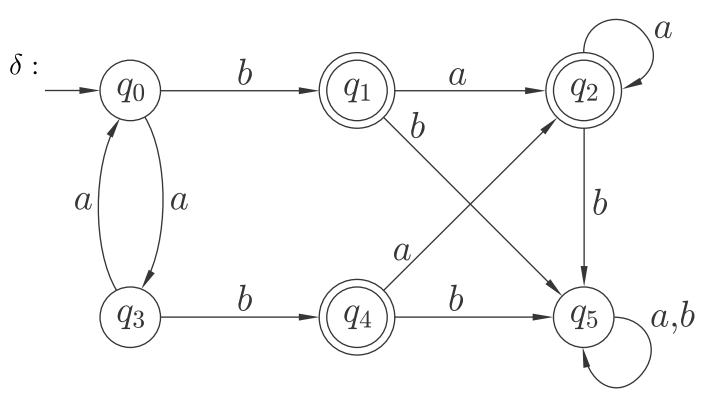
\includegraphics[width=0.8\textwidth]{Blatt9.png}
	\end{center}
\end{figure}

Äquivalenzrelation:
\begin{align*}
	\sim_\A=
\end{align*}

Qutientenautomat $\tilde{\A}$:


\section*{Aufgabe 2}
Gegeben sei der DEA
\begin{align*}
	\A=\Big(\lbrace q_0,\ldots,q_8\rbrace,\lbrace a,b\rbrace, q_0,\delta,\lbrace q_3,q_6\rbrace\Big)
\end{align*}
mit
\begin{figure}[H] 
	\begin{center}
		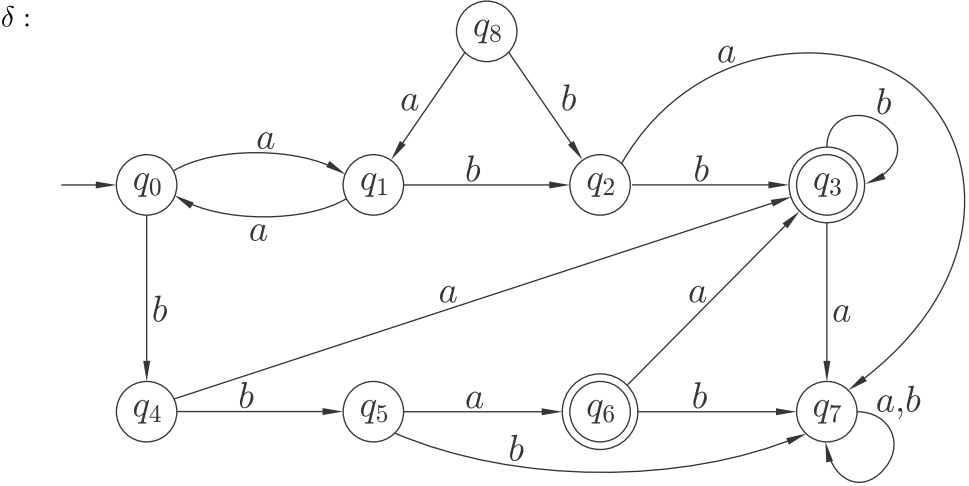
\includegraphics[width=0.8\textwidth]{Blatt9_2.png}
	\end{center}
\end{figure}

Der zu $\A$ reduzierte DEA $\A_{\text{red}}$ ist:
%TODO

\section*{Aufgabe 3}
\subsection*{Aufgabe 3 a)}


\subsection*{Aufgabe 3 b)}


\subsection*{Aufgabe 3 c)}


\end{document}